\documentclass[conference]{IEEEtran}
\IEEEoverridecommandlockouts
% The preceding line is only needed to identify funding in the first footnote. If that is unneeded, please comment it out.

\usepackage{cite}
\usepackage{algorithmic}
\usepackage{graphicx}
\usepackage{textcomp}
\usepackage{xcolor}


\usepackage{mdframed}
\usepackage{hyperref}
\usepackage[underline=true]{pgf-umlsd}
\usepackage{listings}
\usepackage{color}

\usepackage{amsmath,amssymb,amsfonts,amsthm}
\usepackage[english]{babel}
\usepackage[utf8]{inputenc}
\usepackage{algorithm}
\usepackage{adjustbox}
\usepackage{bibnames}
\usepackage{empheq}
\usepackage[title]{appendix}
\usepackage[noend]{algpseudocode}
\usepackage{listings}
\usepackage{mathtools}
\usepackage{float}
\usepackage{enumitem}
\usepackage{graphicx}
\usepackage{textcomp}
\usepackage{xcolor}
\usepackage{varwidth}

\usepackage{tikz}
\tikzset{
  font={\fontsize{8pt}{10}\selectfont}}
\usetikzlibrary{arrows.meta,
                calc, chains,
                quotes,
                positioning,
                shapes.geometric}
  

\usepackage{hyperref}
\usepackage{minted}
\usepackage{caption}
\usepackage{listings}
\usepackage{multirow,array}
\usepackage[super]{nth}
\usepackage[colorinlistoftodos]{todonotes}
\usepackage[font={small,bf}]{caption}
\renewcommand\lstlistingname{Transaction}
\newcommand{\htlctxn}{\texttt{HTLC\_TXN}}
\newcommand{\sellertxn}{\texttt{SELLER\_TXN}}
\newcommand{\bribetxn}{\texttt{BRIBE\_TXN}}
\newcommand{\refundtxn}{\texttt{REFUND\_TXN}}
\newcommand{\refuse}{\emph{refuse}}
\newcommand{\follow}{\emph{follow}}
\newcommand{\strong}{\emph{strong}}
\newcommand{\weak}{\emph{weak}}
\newcommand*\phantomrel[1]{\mathrel{\phantom{#1}}}% My preferred typesetting

\pagestyle{plain}
\floatstyle{boxed}
\restylefloat{figure}


\def\BibTeX{{\rm B\kern-.05em{\sc i\kern-.025em b}\kern-.08em
    T\kern-.1667em\lower.7ex\hbox{E}\kern-.125emX}}
\begin{document}

\title{TWAP Oracle Attacks: Easier Done than Said?}

\author{\IEEEauthorblockN{Torgin Mackinga}
\IEEEauthorblockA{ETH Z{\"u}rich}
\and
\IEEEauthorblockN{Tejaswi Nadahalli}
\IEEEauthorblockA{ETH Z{\"u}rich}
\and
\IEEEauthorblockN{Roger Wattenhofer}
\IEEEauthorblockA{ETH Z{\"u}rich}}


\maketitle

\begin{abstract}
Blockchain ``on-chain'' oracles are critical to the functioning of many Decentralized Finance (DeFi) protocols. We analyze these oracles for manipulation resistance. Specifically, we analyze the cost of manipulating on-chain time-weighted average price (TWAP) oracles. It has been assumed that manipulating a TWAP oracle with the well-known multi-block attack is expensive and scales linearly with the length of the TWAP. We question this assumption with two novel results. First, we describe a single-block attack that works under the same setting as the multi-block attack but whose cost scales with the square root of the length of the TWAP. Second, we describe a multi-block MEV (MMEV) style attack where the attacker colludes with a miner/proposer who can mine/propose two blocks in a row. This MMEV style attack makes oracle manipulation orders of magnitude cheaper than previously known attacks. In the proof-of-work setting, MMEV can be done by selfish mining with very low shares of hashpower.
\end{abstract}

\begin{IEEEkeywords}
TWAP, Oracles, DeFi, MEV, MMEV
\end{IEEEkeywords}

\section{Introduction}
Smart contract platforms such as Ethereum \cite{wood2014ethereum} have allowed for the creation of decentralized finance (DeFi), which aims to recreate financial services such as lending \cite{leshner2019compound,AaveWhitepaper}, exchanges \cite{Zhang2018UniV1,warren20170x}, asset management \cite{yearn_finance,convex_finance}, insurance \cite{KarpNexusMutual}, and more in a fully transparent, trustless, and censorship-resistant way. The total value locked in DeFi has grown to \$108 billion as of December 2021 \cite{DeFiPulse}. Lending and (decentralized) exchange protocols lead the DeFi ecosystem with lending protocols locking around \$51 billion and exchanges locking around \$33 billion in assets. Lending protocols and exchanges enable each other in a bi-directional relationship, with exchanges informing lending protocols about exchange rates and lending protocols providing liquidity to exchanges. The former relationship is often called an \textit{oracle}, where the exchange acts as an oracle and provides market data to the lending protocol. In the rest of this paper, we see how this oracle can be manipulated by sophisticated users to the detriment of the normal users of the lending protocol.

\subsection{Lending}
Lending protocols are smart contracts that allow borrowers to borrow funds at an interest rate. The borrowed assets come from a pool of assets that creditors have deposited as their investments. If this pool suffers a loss due to a bad debt, the loss is distributed among these creditors. If the borrower pays back the debt on time, the interest is divided among the creditors who contributed to the pool from which the loan was made from. Due to the inability of these protocols to take action against loan defaulters (borrowers are just public keys on a blockchain), they use \textit{over-collateralization} to keep the protocols liquid. The borrower first deposits $a$ units of collateral of asset $A$ (with dollar value $V_A$ per unit) and then borrows $b$ units of some other asset $B$ (with dollar value $V_B$ per unit), with $$a\cdot V_A > b\cdot V_B$$ 

Collateralization ratio ($C$) is defined as $C = \frac{a\cdot V_A}{b\cdot V_B}$. If the borrower does not repay the loan on time, the protocol allows any liquidator (a disinterested third party observing the blockchain) to pay back the the borrowed asset and redeem the collateral for the liquidator. For this to be effective, $C$ during the period of the loan should not fall far below the $C$ that the loan started off with. This can happen if the collateral loses value relative to the borrowed asset or the borrowed asset appreciates against the collateral asset. As $C$ tends closer to 1, the lending protocol tries to use the remaining collateral value to make itself whole again with respect to the borrowed asset. Before a loan gets fully undercollateralized ($C < 1$) it can go through a period of ``bad health", where its $C$ has fallen from the time when the loan was made and is now closer to 1 (with some tolerance). To avoid the risk of going fully undercollateralized, the protocol offers liquidators a chance to pay back the loan at a discount, and redeem the remaining collateral for themselves. This makes the protocol whole again, the liquidator gets collateral for a slightly cheaper price, and the borrower is liquidated. The borrower is thus motivated to ``top-up" the collateral to make sure that the loan's $C$ never dips below 1.

Over-collateralization can work only if the lending protocol knows the dollar values $V_a$, $V_b$ of assets $A$, $B$. These assets are traded on many centralized exchanges which operate in the real world, outside of the blockchain. Through trusted third parties, it is possible to get these exchange rates into the lending protocol. These trusted third parties are also called \textit{off-chain oracles}. They are dependent on a trusted third party, so they are not fully \textit{on-chain}. Their operation is not fully governed by a smart contract that can be audited by users and about which users can have assurances of immutability. Lending protocols, which are themselves deployed as auditable smart contracts on-chain, could prefer on-chain oracles, which are deployed as smart contracts, but can still report market-based exchange rates of assets. Automated market makers (AMMs), a type of exchange, serve as a natural on-chain price oracle. They support trades between many pairs of assets and can report the relative exchange rates between asset pairs through state variables available on-chain. 

\subsection{Constant Function Automated Market Makers}
Constant Function AMMs \cite{Zhang2018UniV1} are a type of decentralized exchange that uses a well-known, simple formula to trade one asset for another. An AMM trading pair is a liquidity pool containing reserves $R_A, R_B$ of two different assets $A$ and $B$. If the AMM is using the constant product model, the reserves have a constant product $R_A \cdot R_B = K$. There is a percentage fee $(1 - \gamma)$ that is collected for every trade. When a user sells $b$ units of $B$, they get $a$ units of $A$ such that the constant-product function $(R_B + \gamma \cdot b) (R_A - a) = K$ is preserved. The spot price of asset $A$ is given by $\frac{R_A}{R_B}$, the spot price of asset $B$ is $\frac{R_B}{R_A}$. To see how an entirely on-chain artifact like the ratio of the size of two pools can reflect the \textit{true market price} ($m_p$) of an asset, we have to look at arbitrageurs who constantly watch AMM liquidity pools and other exchanges. Whenever the AMM price deviates from $m_p$, there is an arbitrage opportunity. An arbitrageur could buy assets on the cheaper market, then sell them immediately on the more expensive market for a risk-free profit. In an efficient market, no such arbitrage opportunities should exist, and price imbalances are quickly resolved. The no-arbitrage condition describes a market in which no arbitrage opportunities exist.  Assuming the no-arbitrage condition holds, Angeris et al. \cite{angeris2019uniswap} show that the Uniswap V2 market price deviates from $m_p$ by at most $(1-\gamma)m_p$. If the AMM smart contract makes the ratio $\frac{R_A}{R_B}$ available to be read by other smart contracts, lending protocols can use Constant Function AMM's like Uniswap V2 as their oracles to build over-collateralization mechanisms using artifacts that are entirely on-chain.

\section{Attacks}
During the lifetime of a loan, there is complex interplay between creditors, the lender, the liquidator, the lending smart contract, and the AMM oracle. If the on-chain price of the collateral can be manipulated by a bad actor, the bad actor can also dub as a lender or liquidator to exploit the lending smart contract to make excess profits at the expense of the creditors. In the next sections, we describe two such attacks.

\subsection{Undercollateralized loan attack \label{SectionUndercollAttack}}
A bad actor assumes the role of a borrower to execute this attack. We define the collateral factor $f$ (ranging from 0 to 1) of an asset $A$ as the ratio that governs how much value can be borrowed against $A$. If one deposits $a$ units of collateral $A$ at price $V_A$, they have a \textit{borrowing capacity} of $B_c = f \cdot a \cdot V_A$. Let $m_p$ be the true market price of $A$ and $\epsilon > 0$ be an arbitrary constant. The attacker does the following steps:
\begin{enumerate}
    \item Set aside capital $C$ for the attack. Divide the capital into two piles $C_c$ and $C_m$, such that $C_c + C_m = C$ ($C_c$ is the capital cost and $C_m$ is the manipulation cost). 
    \item \label{step_buy_asset} Using $C_c$, purchase an amount $a$ of asset $A$ at price $m_p$ from any unrelated exchange. $C_c = a \cdot m_p$.
    \item \label{step_manipulate} Using $C_m$, manipulate the AMM price oracle to report the price of $A$ as $(1 + \epsilon) \cdot m_p$ by purchasing an amount $a$ of $A$ on the AMM.
    \item Deposit $a$ of $A$ (bought in step \ref{step_buy_asset}) as collateral and borrow another asset $B$ up to the borrowing capacity $f \cdot a \cdot (1 + \epsilon)\cdot m_p$. If $(1 + \epsilon) > \frac{1}{f}$, this is an under-collateralized loan.
    \item Never pay back the loan. Sell $a \cdot (1 + \epsilon)\cdot m_p \cdot f$ worth of $B$ and book profit $P$.
    \item \label{step_de_manipulate} (Optional) ``De-manipulate" the price of $A$ on the AMM back to $m_p$, receiving back $C_m$.
\end{enumerate}
To simplify, we set $1+\epsilon = \frac{1 + \delta}{f}$, with $\delta$ being another arbitrary constant. The collateral factor $f$ cancels out. Step \ref{step_de_manipulate} can be difficult to do in practice due to frontrunning by arbitrageurs.
Assuming the attacker can do step \ref{step_de_manipulate}, the manipulation has no cost:
\begin{align*}
\begin{split}
    P &= a\cdot(\delta+1)\cdot m_p - C_c, \\
    P &= \delta\cdot C_c.
\end{split}
\end{align*}
Assuming the attacker does not do step \ref{step_de_manipulate}, we have:
\begin{align*}
\begin{split}
    P &= a\cdot(\delta+1)\cdot m_p - C_c - C_m + x \cdot m_p\\
    P &> \delta\cdot C_c - C_m.
\end{split}
\end{align*}

In this case, any attack with $\delta \cdot C_c > C_m$ has a positive profit. To disincentivize such an attack, $C_m$ needs to be high for non-negligible positive values of $\delta$ ($\epsilon$ is linearly related to $\delta$). Oracle designs try to keep $C_m$ high and to make it difficult to execute step \ref{step_de_manipulate}. In further sections, where we look at such oracle designs, we do not consider $C_c$, as it is fully under the attacker's control. We only consider $C_m$ for various values of $\epsilon$. In general, $C_m$ increases with higher $\epsilon$. Larger manipulations are more expensive than smaller ones.

\subsection{Liquidation Attack}
A bad actor assumes the role of a liquidator to execute this attack. In a typical loan, collateral asset $A$ is backing the loan asset $B$. The loan can be made to appear to be in ``bad health" by manipulating the price of $A$ lower or the price of $B$ higher. The oracle, which feeds the price ratio of $A$ vs. $B$ to the lending protocol, has to be manipulated to give the impression to the lending protocol that the price of $A$ has gone lower with respect to the price of $B$. The smart contract will then allow liquidators to settle the loan back in asset $B$ and take asset $A$ out of the protocol, and the liquidator who manages to get this transaction confirmed will successfully make a profit. The attacker does the following steps:
\begin{enumerate}
    \item Set aside capital $C$ for the attack. Divide the capital into two piles $C_c$ and $C_m$, such that $C_c + C_m = C$ ($C_c$ is the capital cost and $C_m$ is the manipulation cost). 
    \item \label{step_buy_asset_liq} Using $C_c$, purchase an amount $b$ of asset $B$ at price $m_p$ from any unrelated exchange. $C_c = b \cdot m_p$.
    \item \label{step_manipulate_liq} Using $C_m$, manipulate the AMM price oracle to report the price of $B$ as $(1 + \epsilon) \cdot m_p$ by purchasing an amount $b$ of $B$ on the AMM.
    \item Choose a loan $L$ from the blockchain which gets below the ``bad health" threshold due to the price of $B$ being $(1 + \epsilon) \cdot m_p$. 
    \item Pay back $b$ units of $B$ to this loan, and get back $a$ units of collateral asset $A$ as liquidation, and book profit $P$.
    \item \label{step_de_manipulate_liq} (Optional) ``De-manipulate" the price of $A$ on the AMM back to $m_p$, receiving back $C_m$.
\end{enumerate}

\subsection{Spot Price Manipulation}
In the attack described in Section \ref{SectionUndercollAttack}, the attacker manipulates the price of an asset on the lending protocol's reference AMM. If the lending protocol uses the naive spot price of an asset as per its AMM, it is straightforward to manipulate this spot price.
In this case, all of the steps in Section \ref{SectionUndercollAttack}, including step \ref{step_manipulate} (the manipulate step), and step \ref{step_de_manipulate} (the de-manipulate step) can be done atomically in a single blockchain transaction. Atomicity ensures that arbitrageurs cannot front-run the attacker's de-manipulate transaction, guaranteeing that step \ref{step_de_manipulate} can be executed successfully. This makes the manipulation cheap. To make matters even worse, the manipulate and de-manipulate steps can be funded by a so-called ``flash-loan" \cite{qin2021attacking}. Flash loans are when a lending protocol lets users borrow large amounts of assets without collateral if they are returned back in the same transaction with small interest and fees. These flash loans remove the capital requirement $C$. This type of naive attack is thwarted by well-known AMMs like Uniswap \cite{Adams2020UniV2} by not allowing spot prices of assets to be recorded in the middle of a block and only recording the price value at the end of a block. This forces the manipulate and de-manipulate steps into different blocks, and flash-loans are no longer an option. Additionally, the de-manipulate step can be front-run by arbitrageurs who notice the manipulate step and want to make a profit by bringing back the manipulated price to the true market price $m_p$. This effect can be made even stronger by not only relying on the price recorded in one block but across many blocks in sequence, leading to the Time-Weighted Average Price (TWAP) oracle.

\section{TWAP oracles}
TWAP oracles double down on the effect mentioned in the previous section, allowing arbitrageurs to front-run de-manipulating transactions so as to keep the manipulation expensive for the attacker. If the classic AMM price is read by the lending protocol, we get the advantage of having the two-block defense against attackers, where the attacker has to manipulate the price in a block and wait for the next block to de-manipulate the price. If we extend this to multiple blocks, where the lending protocol reads the price of an asset averaged over many blocks, the attacker has to keep the manipulation going for that duration and pay the price for it.

One example of an on-chain price oracle is the Uniswap V2 oracle \cite{Adams2020UniV2}. It records the price of a particular Uniswap V2 trading pair's smart contract before the first trade of each block. This price, multiplied by the number of seconds that have passed since the last update, is observation $p_i$. All observations get stored in an accumulator $a_t$ with
\begin{align*}
    a_t = \sum_{i=1}^{t}p_i.
\end{align*}

The accumulator should always reflect the sum of the spot price at each second in the history of the contract.
An external caller (the lending protocol, for example) can checkpoint the accumulator's value at time $t_1$, then again at $t_2$. Using these values, it calculates a time-weighted average price, or TWAP, from $t_1$ to $t_2$ as:
\begin{align*}
    \text{TWAP}_{t_1,t_2} = \frac{a_{t_2} - a_{t_1}}{t_2 - t_1} 
\end{align*}

Taking an average over many blocks allows arbitrageurs more time to successfully front-run an attacker's de-manipulation transaction. In the worst case for the attacker, arbitrageurs will front-run the de-manipulation transaction in every block. TWAP oracles have a clear tradeoff between manipulation resistance and freshness. Using a larger $(t_2 - t_1)$ in the TWAP increases the cost of manipulation, while a shorter TWAP follows the spot price more closely. Using a longer duration TWAP comes with the risk of the TWAP not reflecting the true spot price of an asset, and the lending protocol not responding to real market conditions that cause loans to get under-collateralized. 

\subsection{TWAP manipulation cost}
Let $m_p$ be the true market price of an asset $A$. Let $\epsilon > 0$ be some desired constant on which we want to parameterize the cost of manipulation $C_1$ of $A$ for just one block to the new price $(1+\epsilon)\cdot m_p$. Angeris et al. \cite{angeris2019uniswap} have shown this cost to be:
\begin{align*}
    C_1(\epsilon) = R_B(\sqrt{1+\epsilon} + (\sqrt{1+\epsilon})^{-1} -2)
\end{align*}
where $R_B$ is the Uniswap V2 trading pair's liquidity reserve of asset $B$. This assumes no fees, an infinitely liquid reference market, and the no-arbitrage condition. Increasing the market price of $A$ is equivalent to lowering the market price of $B$, so this result can also be used for the case where a manipulator wants to lower the price of an asset. 

The same paper shows that $C_1(\epsilon)$ can be bounded from below by:
\begin{align}
    C_1(\epsilon) \geq K R_{B} \min\{\epsilon^2, \sqrt{\epsilon}\}
    \label{AngerisCostBound}
\end{align}
where $K > 0$ is a universal constant. This shows that for $\epsilon \leq 1$, cost scales with $\epsilon^2$, for $\epsilon > 1$ it scales with $\sqrt{\epsilon}$.
Independently of $\epsilon$, cost also scales linearly with liquidity. $C_1$ is the cost for the attacker to manipulate the oracle for a single block. If a TWAP is being used by the lending protocol, to pull off the under-collateralized loan attack from Section \ref{SectionUndercollAttack}, the attacker must keep this manipulation for multiple blocks $L_T$, where $L_T$ is the length of the TWAP. The total cost of the multi-block attack is $C_m = L_T \cdot C_1(\epsilon)$. The cost $C_1(\epsilon)$ is incurred as arbitrage loss every time an arbitrageur de-manipulates the price instead of the attacker. This result (\ref{AngerisCostBound}) has led to the generally accepted conclusion that ``the cost of manipulating the Uniswap price [oracle] to any fixed amount scales linearly with the reserves and the number of blocks" \cite{AngerisMedium}. Next, we show with our first novel result that an AMM-based price oracle can be manipulated for higher profits with lower costs.

\subsection{Single-block attack}
In the (safely expensive given large liquidity reserves) multi-block attack model, optimistic users assume that the attacker needs to pay a huge price to manipulate $m_p$ to $(1+\epsilon)\cdot m_p$ over $L_T$ successive blocks. Our insight is that the same effect can be seen if the attacker can manipulate $m_p$ for just one block to $(1 + L_T \cdot \epsilon) \cdot m_p$. We call this the single-block attack. Assuming the price is $m_p$ in all other blocks, the oracle will report a price of $\frac{ L_{T} + L_T \cdot \epsilon}{L_{T}}\cdot m_p = (1+\epsilon)\cdot m_p$, just like the multi-block attack. The cost of manipulation for the single-block attack is given by $C_1(L_T \cdot \epsilon)$, while the multi-block attack had cost $L_T \cdot C_1(\epsilon)$. From the bound in Equation (\ref{AngerisCostBound}), we can deduce that $C_1(L_T\cdot\epsilon)$ scales with $\sqrt{L_T\cdot\epsilon}$. The single-block attack is cheaper when
\begin{align*}
   C_1(L_T \cdot \epsilon) < L_T \cdot C_1(\epsilon)
\end{align*}

The single-block attack will be cheaper than the multi-block attack at some value of $L_T$. To find this, we solve (\ref{OneBlockCheaperEq}) for $L_T$. This results in
\begin{align*}
    L_T > \frac{4 (2+2 \epsilon+2 \sqrt{1+\epsilon}+\epsilon \sqrt{1+\epsilon})}{\epsilon^3}.
\end{align*}
The dominating term on the right-hand side of the inequality is $\epsilon^3$. If $\epsilon$ is small, $L_T$ needs to be large. For large $\epsilon$, even a small $L_T$ is sufficient. Figure \ref{figureCostDiff} shows the ratio of multi-block attack cost divided by single-block attack cost. It scales with the square root of $L_T \cdot \epsilon$, which is expected as $\frac{L_T \cdot \epsilon}{\sqrt{L_T \cdot \epsilon}} = \sqrt{L_T \cdot \epsilon}$.

\begin{figure}[h]
\centering{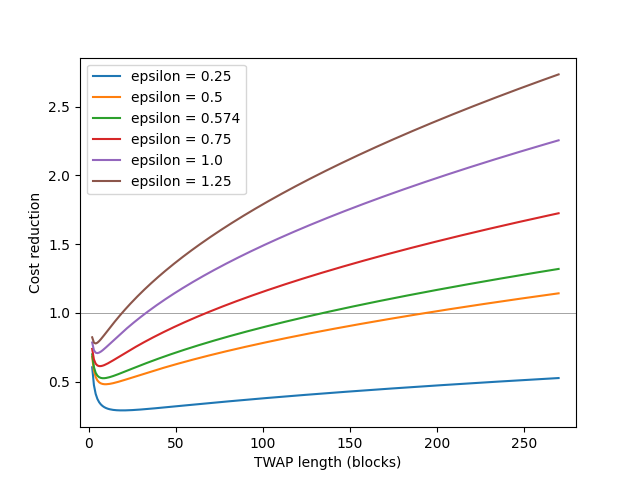
\includegraphics[scale=0.5]{figures/Cost difference.png}}
\caption{Cost comparison between the multi-block and single-block attack. The y-axis shows how much cheaper the single-block attack is. The single-block attack is more expensive when the cost reduction is less than 1.}
\label{figureCostDiff}
\end{figure}

The break-even point, where both attacks have an equal cost for a 135 block TWAP oracle (which is a commonly used value in practice), is at $\epsilon = 0.574$. For higher $\epsilon$, the single-block attack is cheaper than the multi-block attack. For lower $\epsilon$, it is more expensive. Ironically, an attacker that wants to manipulate an asset's price higher to achieve a larger profit can do so in a proportionately cheaper way.

\subsection{Failed Assumptions}
The idea that the only way to manipulate a TWAP oracle is through the expensive multi-block attack already makes a few assumptions, like the no-arbitrage condition, an infinitely liquid external market for asset $A$ which arbitrageurs can tap into, and that arbitrageurs can always front-run the attacker's de-manipulation transaction. These assumptions have to be true to make the multi-block attack expensive for an attacker, thereby making the TWAP oracle safe to use. If the assumptions do not hold, the multi-block attack might already not be as expensive as previously thought. The single block attack, which is cheaper for larger manipulations, also makes the same assumptions. In this case, the assumptions are even less likely to hold -- thereby making the single block attack even cheaper to execute.

\textbf{No-arbitrage condition:} For the single-block attack, the no-arbitrage assumption is less likely to hold than for the multi-block attack. Arbitrageurs only have a single block to act, ruling out manual arbitrage and forcing bot-based arbitrage. This general-purpose arbitrage bot needs instant access to a large amount of asset $A$. This eliminates all off-chain exchanges as reference markets since it would take at least one block to transfer funds out of the exchange.

\textbf{Infinitely liquid external market:} Eliminating off-chain exchanges also makes the assumption that arbitrageurs have access to an infinitely liquid external market less likely to hold. If arbitrageurs are unable to react within a single block, the manipulation is free.

\textbf{Transaction Ordering:} Transaction ordering within the block is even more important in the single block attack than in the multi-block attack. If the attacker can get a de-manipulation transaction included in the second block before the arbitrageur can, the attack is also free.
\bigskip

Additionally, against a multi-block attack, a DeFi protocol admin has an entire TWAP length to notice that a price is being manipulated and trigger emergency shutdown procedures if they exist. In a single-block attack, the oracle already reports the manipulated price in the very next block, and an exploit can take place immediately with no prior warning. Even if all assumptions hold, the novel result we arrive at is that for large enough $\epsilon$ and $L_T$, the cost of manipulation of a TWAP oracle only scales with the square root, not linearly with the TWAP length. If some of the assumptions do not hold, an attack may be dramatically cheaper than expected. 

In the next section, we look at a scenario where all these safety assumptions fail. The attacker controls a miner/proposer and can propose two blocks in a row: one with the manipulating transaction and one with the de-manipulating transaction. 

\section{Multi-Block MEV}
Miner Extractable Value (MEV) is the value that can be extracted by miners/proposers who order the transactions that go into a block. This ordering gives them the power to include their own transactions ahead of other users' transactions and thereby extract value out of the ordering process, which goes beyond their usual rewards of fees and block subsidies. Daian et al. \cite{daian2019flashboys} first explored the many ways in which transaction ordering can be used to extract more value. If an attacker could specify a transaction ordering over multiple blocks in a row, they would no longer need to compete with arbitrageurs. We call this Multi-block MEV, or MMEV. 

In the proof-of-work setting, it is not known ahead of time which miner will mine the next block. However, if a miner does selfish mining \cite{eyal2014majority,sapirshtein2016optimal,Ritz_2018} and maintains a private chain, they can publish the private chain judiciously to extract more value than their share of hash power would warrant. In our case, the selfish miner has an even simpler goal -- to include their own transactions in two blocks in a row and make these two blocks get into the main blockchain. The MMEV, in this case, is the ability to cheaply manipulate a TWAP oracle, and additionally, also execute an under-collateralized loan attack on a lending protocol that uses this oracle. We show that selfish mining to enable such MMEV is feasible with much lower shares of total hash power than what is traditionally expected for profitable selfish mining. Selfish mining attacks on the Uniswap V2 TWAP oracle are acknowledged in the Uniswap V2 whitepaper \cite{Adams2020UniV2} and its security audit \cite{UniswapAudit}, but has not been studied formally before.

\subsection{Attack Capital}
As before, the total cost of the attack consists of $C_m$, the cost of oracle manipulation, and $C_c$, the capital required to perform the under-collateralized loan attack. First, we assume that the attacker controls the contents of two blocks in a row and is able to execute the single block attack described earlier. This makes $C_m$ reduce to the fees of the AMM, as there are no arbitrageurs to fight off because of selfish mining. Selfish mining itself has a cost that is independent of the attack, and we will look at that in subsequent sections.

The attacker controls two blocks. In the first block, the attacker buys $a$ of asset $A$, increasing the market price to $(1 + L_T \cdot \epsilon) \cdot m_p$, as required by the single block attack. This costs $b$ of asset $B$. In the first transaction in the second block, the attacker sells $a$ units of asset $A$, returning the market price to $m_p$, receiving $b$ units of $B$. Under normal circumstances, the transaction in the first block would be vulnerable to arbitrage. Controlling two consecutive blocks allows an attacker to be immune to arbitrage and makes the manipulation cost reduce to the AMM fee. Note that the under-collateralized loan attack on the lending protocol requires separate capital that is independent of the oracle manipulation cost $C_m$ we are discussing here. An MMEV attack is cheaper than a single-block attack if it is cheaper to create two blocks in a row than being vulnerable to an arbitrage that nullifies the attacker's de-manipulation transaction. The cost of selfishly mining two blocks in a row is fixed. It does not depend on $L_T$ or $\epsilon$. Assuming a constant product AMM like Uniswap, we have $R_A \cdot R_B = K$, we can calculate the required $b$ to achieve a price for $A$ of $(1 + L_T \cdot \epsilon)\cdot m_p$:
\begin{align*}
    b &= \sqrt{1 + L_T \cdot \epsilon}-1.
\end{align*}

Given a 0.3\% swap fee of the AMM, and a TWAP length of 135 blocks (30 minutes, if we assume Ethereum as the smart contract platform), we calculate values of $b$ and swap fees required for different values of $\epsilon$. Table \ref{TableCosts} shows that doubling the TWAP price of $A$ for a 30-minute TWAP (by setting $\epsilon = 1$) on a pair with \$2,000,000 of total liquidity, \$1,000,000 worth of $A$ and $B$ respectively, would cost \$35,000 in AMM fees and require temporary capital of \$10,660,000. Increasing TWAP to $100 \cdot m_p$ (setting $\epsilon = 99$) would cost \$346,000 in AMM fees and require temporary capital of \$114,610,000. The amount of temporary capital required for the manipulation is likely a bigger limiting factor for an attacker than the cost in fees. Note that using a flash loan to acquire the needed funds is not an option, as they are used over two blocks.

\begin{table}[ht]

\begin{center}
 \begin{tabular}{|c |c| c|} 
 \hline
 $\epsilon$ & $b$ & fees\\ [0.5ex] 
 \hline\hline
 0.5 & 7,280,000 & 25,000 \\ 
 \hline
 1 & 10,660,000 & 35,000 \\ 
 \hline
 9 & 33,870,000 & 105,000 \\ 
 \hline
 99 & 114,610,000 & 346,000 \\  
 \hline
\end{tabular}
\end{center}
\caption{Amounts and trading fee costs for different $\epsilon$.}
\label{TableCosts}
\end{table}


\subsection{Selfish Mining Cost\label{sectionSelfishMining}}
Selfish mining cost is given by the opportunity cost of not mining blocks on the main chain. We model the following miner strategy S:
The selfish miner $M$ mines on the main chain until he successfully mines a block $B_{1}$. $M$ does not publish $B_{1}$ and continues mining on top of $B_{1}$.
If $M$ finds a second block $B_{2}$, $M$ immediately publishes both $B_{1}$ and $B_{2}$. $M$'s chain is now longer than the main chain, and all honest miners will continue mining on $M$'s chain. We call this a success. If two blocks are added to the main chain without $M$ finding a block $B_{2}$, $M$ publishes $B_{1}$. This will turn $B_{1}$ into an uncle block. Then $M$ starts over and returns to mining the main chain.

\begin{figure}[h!]
\centering
\begin{tikzpicture}[auto, thick,align=center]
    %states
    \node[state] (0) {$0,0$};
    \node[state,right=of 0] (1) {$1,0$};
    \node[state,below=of 1] (2) {$1,1$};
    \node[state,right=of 1] (3) {$2,x$};
    
    %edges
    \draw [->] (0) edge[loop left] node {$1-p$} (0);
    \draw [->] (0) edge[bend left, auto=left] node {$p$} (1);
    \draw [->] (1) edge[auto=left] node {$1-p$} (2);
    \draw [->] (1) edge[bend left, auto=left] node {$p$} (3);
    \draw [->] (2) edge[bend right, auto=right] node {$p$} (3);
    \draw [->] (2) edge[bend left, auto=left] node {$1-p$} (0);
    \draw [->] (3) edge[loop right] node {$1$} (3);
    
\end{tikzpicture}
\caption{Markov chain model of strategy S}
\label{MarkovFull}
\end{figure}

Let $p$ be the share of the total hash rate that M controls. The probability of M mining any block is $p$, and the probability of all other miners mining that block is $1-p$. We assume that the propagation of newly published blocks to the network is instantaneous. Let $\mathbb{E}[S]$ be the expected number of blocks it takes to have success when following strategy S. We use the Markov chain given in Figure \ref{MarkovFull} to model strategy S. The states of the Markov chain contain pairs of $(n_1,n_2)$ with $n_1=$ number of blocks on the private chain and $n_2=$ number of blocks on the main chain. The absorbing state $(2,x)$ is the state where the selfish miner is leading with the required length 2 and will release both blocks to the main chain. As this is a finite discrete absorbing Markov chain, we can calculate the expected hitting time $\mathbb{E}[S]$ of state $(2,x)$ given the initial state is $(0,0)$ as:

\begin{align*}
    \mathbb{E}[S] = \frac{1 + 2p - p^2}{2p^2 - p^3}
\end{align*}

\noindent
\textbf{Opportunity Cost:} In the original selfish mining research on Bitcoin \cite{eyal2014majority}, the selfish miner forgoes mining rewards if the miner's private blocks do not make it to the main blockchain. In Ethereum, there is a way to reduce this opportunity cost by making these private blocks into public uncle blocks and collect uncle block rewards. It takes $\mathbb{E}[S]$ blocks for MMEV success. During this time, the miner has a $p$ chance of mining a block. This makes their uncle block opportunity $\mathbb{E}[S] \cdot p - 2$. The last two blocks cannot count as uncle blocks as the selfish miner releases them as part of the main blockchain. Uncle blocks mitigate the attack cost even more, at the cost of exposing the possibility that an attack might be happening.

\textbf{Total Cost:} In Ethereum, blocks are generated every 15 seconds, leading to 240 blocks per hour.\footnote{In practice, Ethereum has a slightly faster block generation time of ~260 blocks per hour.} The dollar cost of selfish mining is calculated based on Ethereum's total hash rate of 715 terahashes/s \cite{ethereum_hash_rate}, and the cost of renting hash power at \$60,000 for one terahashes/s for 24 hours \cite{nicehash}. As we see, an attacker can rent 1.5\% hash rate for 9 hours by paying \$258,000 and expect to selfishly mine two blocks in a row. As the MMEV selfish miner has different goals than the traditional selfish miner, a much lower share of the total hash rate is enough for success. This is important because renting a higher hash rate can distort the inelastic hash rate market, and the price per hash will go up. Uncle rewards are reduced by 0.25 ETH for each generation that they are late. We remove 0.25 ETH from the average uncle block reward, putting the uncle block reward at 1.46 ETH. If we look at low values for $p$, the expected time to success (in hours) and the approximate total cost in dollars for the attack are shown in Table \ref{TableHittingTime}.
\break

\begin{table}[h!]
\begin{center}
 \begin{tabular}{|c |c| c | c | c|} 
 \hline
 $p$ & $\mathbb{E}[S]$ in hours & Cost in dollars & Uncle Rewards & Total Cost\\ [0.5ex] 
 \hline
  0.25\% & 335& \$1,499,000 & \$598,000 &\$901,000\\
  \hline
  0.50\% & 84& \$754,000 & \$298,000 &\$456,000\\
  \hline
  0.75\% & 37& \$506,000 & \$198,000 &\$308,000\\
  \hline
  1.00\% & 21& \$382,000 & \$148,000 &\$234,000\\
  \hline
  1.25\% & 13& \$307,000 & \$118,000 &\$189,000\\
  \hline
  1.50\% & 9& \$258,000 & \$98,000 &\$160,000\\
  \hline
\end{tabular}
\end{center}
\caption{Selfish Mining MMEV hash rates, costs, and rewards}
\label{TableHittingTime}
\end{table}

In the proof-of-stake setting \cite{proof_of_stake}, if block proposers are known in advance, two proposers could collude and perform MMEV style oracle manipulation. These attacks do not go against standard consensus rules of blockchains, and hence, it is not clear if validators would slash such colluding proposers. We leave this problem for future research when proof-of-stake algorithms are standardized and seen in larger blockchains like Ethereum.

\section{Results}
We compare the three different TWAP manipulation attacks we have seen so far. We again use the example where we want to double a 30-minute TWAP for a pair with \$2,000,000 of total liquidity reserves. 

\begin{itemize}
    \item[] The cost of the MMEV single-block attack with 1.5\% hash rate is \$160,000.
    \item[] The cost of the single-block attack is $C(135 \cdot 1)$ = \$9,747,653.
    \item[] The cost of the multi-block attack is $135 \cdot C(1)$ = \$16,200,000.
\end{itemize}
 
All attacks ignore the rather small AMM trading fee of around \$35,000. The multi-block attack cost scales linearly with the TWAP length $T_L$, whereas the single-block attack costs only scale with the square root of $T_L$. The MMEV single-block attack avoids this cost entirely as it has no arbitrageurs to worry about. The cost of selfish mining-based MMEV single block attacks only depends on the share of hash power required to pull off the attack in a reasonable time. Even with a conservative estimate of 1.5\%, it is almost two orders of magnitude cheaper than the other attacks.

\subsection{Solution \label{sectionPotentialSolution}}
First, as seen in commentary on Equation (\ref{AngerisCostBound}), an asset pair having high liquidity $R_A, R_B$ makes the costs of the non-MMEV attacks scale linearly with it, which mitigates the attack to some extent. In the MMEV single-block attack, only the cost of trading fees scales with liquidity. For all attacks, the amount of temporary capital required scales linearly with liquidity. Illiquid assets are more likely to get attacked in the ways discussed above. Using a longer length for the TWAP is not ideal mitigation against the standard and MMEV versions of the single-block attack, as the cost and capital requirements only scale with the square root of the TWAP length in the best case. The fundamental issue that these attacks exploit is that a TWAP can be affected significantly by manipulating a single block's price. This could be solved by using a median price instead of an average. A median is largely unaffected by outlier prices in single blocks. This eliminates the single-block attack and requires the MMEV attack to take place over many blocks and not just two. It is important to note that a median is less resilient to the multi-block attack than a TWAP. To manipulate a median, it is sufficient to manipulate only half the blocks it encompasses. Consequently, the multi-block attack becomes cheaper by 50\% if the median is used instead of the average.

Uniswap V3 \cite{Adams2021UniV3} introduces the possibility of having a pair's price stored every block, with up to 65536 checkpoints. Given that there are as many checkpoints as the desired median length, a median could easily be calculated from this data. Calling a median oracle would be significantly more expensive in terms of computation costs (gas fees) than a TWAP oracle, as all checkpoints will need to be loaded from storage to calculate the median. The additional cost is only incurred when calling the oracle's update function. Uniswap V3's base architecture needs no changes in order to support calculating the median. Any protocol that uses Uniswap V3 as its oracle could use a median instead of a TWAP.

\section{Conclusion}
We illustrated the need for a manipulation-resistant oracle with the under-collateralized loan attack on a lending protocol. Any protocol that relies in the same way on a TWAP oracle is vulnerable. We have analyzed the manipulation resistance of TWAP oracles against different types of attacks and showed that the cost of manipulation for TWAP oracles is lower than expected. We introduced the single-block attack, which for longer TWAPs is cheaper to execute than the previously known multi-block attack. Previously, it was assumed that a TWAP oracle is safe because the multi-block attack is expensive to execute because the safeguards against the attack are assumed to work. We show that the single block attack is not only cheaper to execute, but the assumed safeguards do not work. One of the safeguards that the multi-block attack's ``infeasibility bubble" assumed is that arbitrageurs can get assets from external off-chain exchanges to revert the manipulated price back to the market price. The single block attack leaves no time for arbitrageurs to do this, thereby restricting this assumption to just on-chain exchanges.

Another safeguard that the multi-block attack's ``infeasibility bubble" assumed is that arbitrageurs will always arbitrage the manipulated price back to the market price. Under the MMEV setting, we show that if an attacker can mine two blocks in a row, this no-arbitrage condition fails, and the attack gets dramatically cheaper. The area of MMEV is under-explored and should be analyzed for other exploits that are only possible when an attacker controls multiple blocks in a row. 

These attacks do not target a specific victim transaction. The goal is to manipulate an oracle that a DeFi protocol relies upon and exploit the protocol. A protocol's structural reliance on an oracle does not change much with time, and this attack is always available for the taking, based on the attacker's ability to acquire capital to pull off the attack.

As a solution, we also suggest that TWAP oracles should rather use the median as a manipulation-resistant statistic instead of a mean. An interesting open research question is to find novel sampling techniques of Uniswap V3's price checkpoints to get a manipulation resistant statistic other than the median or mean that also responds quickly to an asset's true market price.

\bibliographystyle{IEEEtran}
\bibliography{references}
\end{document}
